\section{Compact Muon Solenoid}
\label{sec:Exp_CMS}
\subsection{Introduction}

The CMS is a general-purpose detector designed for detecting various highly energetic particles which are being produced in $pp$ collisions at the LHC~\cite{ref_CMS_TDR}. The CMS has a broad program with goals of direct and indirect searches of the BSM physics including but not limited to supersymmetric particles as well as precision measurements of various SM parameters. 

% MAY NOT NEED THIS SENTENCE HERE
%Its main feature is a large magnet to create a magnetic field of~4T to curve charged particles in the tracking system and of~2T outside to curve muons in the muon system.

The CMS detector is a cylindrically symmetric with a colliding beam as a central axis. Cartesian, cylindrical and spherical coordinates are all used to describe the CMS geometry, depending on the context. The $x$-axis of the CMS points towards the center of the LHC while the $y$-axis points vertically up. The direction of the $z$-axis corresponds to the couterclockwise direction of the LHC beam (Fig.~\ref{fig:CMScoord}, left). Cylindrical coordinates are defined as $r=\sqrt{x^2+y^2}$, $\phi=arctan(y/x)$. Instead of the polar angle $\theta$, it is more convinient to use the pseudorapidity $\eta=-\ln{\tan{\theta/2}}$. A pseudorapidity ranges from $\eta=-\infty$ to $\eta=+\infty$ for directions parallel to the beam axis with the value of $\eta=0$ for a direction perpendicular to the beamline. This variable is convinient for measurements because a distribution of a massless particle in $\eta$ is nearly flat. The acceptance of the CMS in $\eta$ is limited and varies from $|\eta|<2.4$ to $|\eta|<5.0$ depending on a subdetector (Fig.~\ref{fig:CMScoord}, right).   

\begin{figure}[htb]
  \begin{center}
    {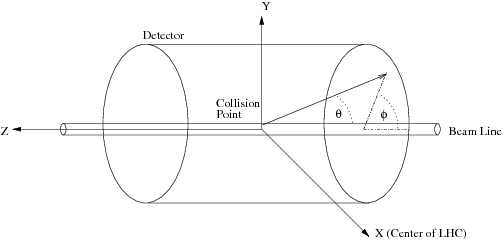
\includegraphics[width=0.45\textwidth]{../figs/Exp/CMScoord.png}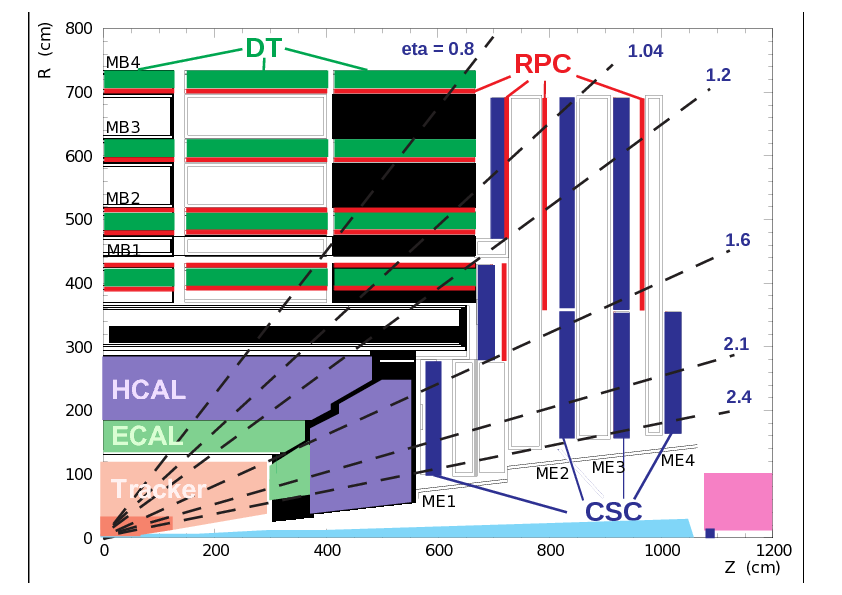
\includegraphics[width=0.45\textwidth]{../figs/Exp/CMScoord_eta.png}}
    \caption{Left: CMS coordinate system. Right: pseudorapidity ranges for different CMS subdetectors.}
    \label{fig:CMScoord}
  \end{center}
\end{figure}

The detector consists, from inner to outer layer,  of a tracking system, an electromagnetic calorimeter (ECal), a hadronic calorimeter (HCal), a magnet and a muon system. Having the tracking system, ECal and HCal inside of a large solenoid makes the detector compact. A segment of a CMS slice in $r-\phi$ plane is shown in Fig.~\ref{fig:CMS_slice}.

EXPLAIN WHAT IS TRACK

EXPLAIN WHAT IS PRIMARY VERTEX (HERE?)

When a heavy particle is produced in a collision, it decays immediately, and we detect its long-living decay products including an electron, a photon, a muon, a neutral hadron or a charged hadron. Depending on the trace left by a particle in different subdetectors we can identify a particle. Electrons and positrons leave curved tracks in the tracking system and then induce showers in the electromagnetic calorimeter (ECal). Photons induce the same electromagnetic showers is ECal however, as neutral particles, they do not leave tracks in the tracking system. Hadrons normally travel through the ECal undisturbed and induce a hadronic shower in the hadronic calorimeter (HCal). Charged and neutral hadrons can be distinguished from each other by checking whether they leave a track in the tracking system or not. Muons are the only particles which penetrate through the ECal, the HCal and the magnet and leave tracks in the CMS muon system. Neutrinos are not detected by CMS.   

\begin{figure}[htb]
  \begin{center}
    {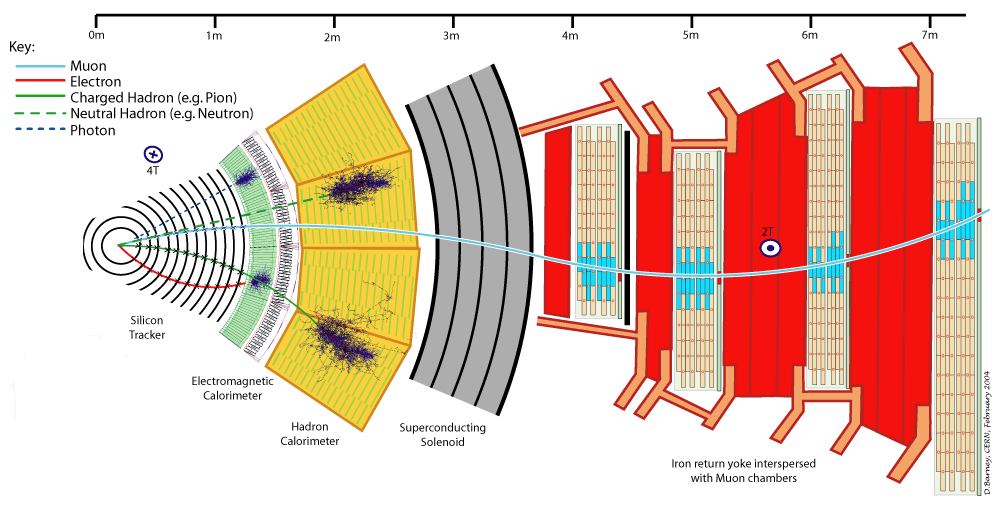
\includegraphics[width=0.98\textwidth]{../figs/Exp/CMS_Slice.png}}
    \caption{CMS slice.}
    \label{fig:CMS_slice}
  \end{center}
\end{figure}

% CMS detector geometry and variables

% In this dissertation...
All subdetectors are important for the $W\gamma$ measurement and the remainder of this chapter describes the subdetectors in greater details. Muons and electrons which we have as final state particles are both affected by CMS magnetic field allowing the tracking system and the muon system to measure their trajectory parameters and momenta. In this dissertation we use the information of the primary vertex determined by the tracking system to select our events. Also the tracker provide us the information about electrons trajectories and momenta in the electron channel and distinguishes between electrons and photons. The ECal is necessary to identify electrons and photons and to measure all kinematic parameters of photon. The HCal is also used for electrons and photons identification: the energy deposit in the HCal left by an electron or a photon must be very small compared to the energy deposit left in the ECal. The muon system is essential for muon reconstruction and identification.

\subsection{Magnet}

% CONTENT-WISE IS OK

A magnetic field in a particle detector is necessary to measure momenta of charged particles by track curvatures. The higher the momentum is, the less a particle trajectory is affected by the magnetic field. In CMS momenta of all charged particles are measured in the tracking system. In addition, momenta of muons are measured in the muon system. 

The CMS magnet is placed between layers of HCal and a muon system. The magnet is made of superconducting wires. An electric current flowing in the wires creates a uniform field of $B=4$T inside the solenoid, for the tracking system, and also provides a smaller magnetic field of a certain configuration outside the solenoid, for the muon system. Stronger field in the tracking system is necessary because of higher track density and a smaller size than those in the muon system.

\subsection{Tracking System}

%WHAT IS HIT

%COLLISION TRACKS

%"The tracker is designed in such a way that a single track hits multiple sensors."

%    "Then the trajectory is reconstructed based on how much charge is collected on each sensor."

%       What does it mean, exactly, each of these sentences? It is not clear to me.

The tracking system measures track geometry including particles trajectories and locations of primary and secondary vertices and momenta of charged particles. It needs to disturb particles as little as possible so that they can pass through. Therefore, just a few measurements must be enough to reconstruct the track. The accuracy of a measurement of each hit is~10~$\mu$m.

The tracking system consists of silicon pixels and silicon strips (Fig.~\ref{fig:tracker_slice}). Collision tracks start at the center and then cross the layers of the tracking system. Tracks are straight in $r-z$ plane and curved by the magnetic field in the $r-\phi$ plane. The acceptance of the tracker system in $r-z$ plane is geometrically limited by the absolute value of the pseudorapidity $|\eta|=2.5$.

The pixel tracker is the closest subsystem of CMS to the collision point thus it experiences the largest particle flux: at~8~cm from the collision point the flux is about~10~million~1/(cm$^2$s), and the pixel detector with its~65~millions sensors is capable to reconsruct all these tracks. It consists of three layers of cylinders in the barrel with radii of~4~cm,~7~cm and~11~cm which are referred as pixel barrel (BPIX) and four disks in the endcap, two disks at each side, which are referred as pixel forward (FPIX). The tracker is designed in such a way that a single track hits multiple sensors. Then the trajectory is reconstructed based on how much charge is collected on each sensor. This allows us to reach a spacial resolution of 15-20~$\mu$m which is much smaller than a distance between sensors.

The strip tracker is placed right after the pixel tracker and occupies the detector volume up to~130~cm around the beam axis. The strip tracker consists of four parts: the tracker inner barrel (TIB), the tracker inner disks (TID), the tracker outer barrel (TOB) and the tracker endcap (TEC) as shown in Fig.~\ref{fig:tracker_slice}. In the strip tracker there are over 15,000 sensitive modules with a total number of~10~million strips. Each sensitive module consists of a set of sensors, its support structure and readout elements.

%electric charge and amplification

%limitations

\begin{figure}[htb]
  \begin{center}
    {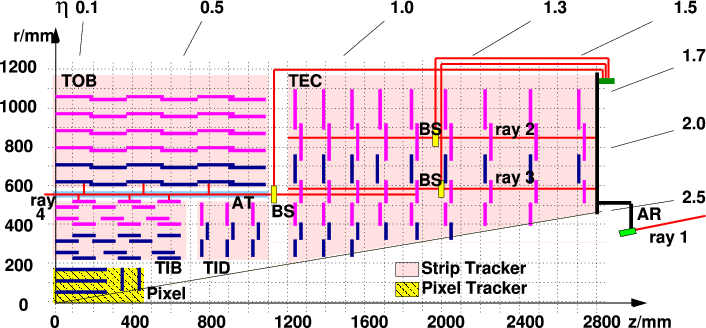
\includegraphics[width=0.8\textwidth]{../figs/Exp/tracker_slice.png}}
    \caption{Slice of the CMS tracking system in $r-z$ plane.}
    \label{fig:tracker_slice}
  \end{center}
\end{figure}

\subsection{Electromagnetic Calorimeter}

The ECal is a layer between the tracking system and the HCal. It is made of high-density lead tungstate crystals arranged in a barrel section and two endcap sections. The crystals work as scintillators. When electrons and photons pass through it, it produces light proportional to the particle's energy. The scintillated light then is amplified by photomultipliers producing signals on sensitive elements.

Thus, the ECal measures energy of electrons and photons and parameters of their trajectories. To distinguish between electrons and photons, it is necessary to perform matching to the track in the tracking system. If there is a track, then there is an electron (or positron). If there is no track, then the particle is a photon.

It is important for the ECal to be able to distinguish between high energetic photons and pairs of lower energetic photons e.g. from a $\pi^0$ decay. It is especially difficult in the endcap sections where angle between two photon trajectories is small. For this reason, ECal preshowers which have~\~15~times smaller granularity are located in front of the endcaps. The preshowers provide extra spacial precision. 

%Their strips are~2~mm wide compared to~3~cm wide crystals in the main volume of the ECal.

%(Why muons and hadrons don't release their energy here?)
%limitations

\subsection{Hadron Calorimeter}

The HCal is placed right after the ECal and is the last subdetector within the magnet. The HCal measures energies of charged and neutral hadrons. In addition, the HCal determines the track parameters. Match to the tracking system has to be done: if a matching track found, then it is a chagred hadron otherwise it is a neutral hadron. 
%(Why muons don't release their energy here? Would photons and electrons release the energy here?)

The HCal consists of alternate layers of absorbers and scintillators. Hadrons hit brass or steel plate of absorber producing secondary particles. When emerge into the scintillator, the particles induce hadronic and electromagnetic showers and emit blue-violet light which is further shifted to the green region and read out by special boxes within the HCal. The secondary hadrons produced during the interaction with the absorber interact with the next absorber producing more showers in the next layers of scintillators and also affect the total enegry deposit. All hadrons must be stopped inside the layers of the HCal.

%HCal Sampling calorimeter (?)
%Hybrid Photodiodes

\subsection{Muon System}

Muons pass through the ECal, the HCal and the magnet without interacting. They are the only particles that are registered in the muon system which is placed outside the magnet and which is the largest part of CMS detector.

There are four concentric layers of muon detectors (stations) and iron return yoke between them. Muons induce several hits in the muon stations which are later fitted and matched to the tracking system measurements to provide the best possible resolution in the measurements of all parameters of the muon's trajectory and momentum.

There are three types of muon chambers used in the CMS muon system: drift tubes (DTs), cathode strip chambers (CSCs) and resistive plate chambers (RPCs). Overall, there are 1400 muon chambers including 250 DTs, 540 CSCs and 610 RPCs.

The system of DTs measures positions of muons in the barrel. Each DT chamber is about~2~m by~2.5~m in size. It consists of~12~layers of aluminium which are arranged as groups of four. There are up to~60~drift tubes in a layer. The middle group of layers measures $z$-coordinate and two other groups determine the perpendicular coordinate.

Each drift tube is~4~cm in width, is filled with a gas and has a wire inside. When a charged particle passes through the volume, it ionizes atoms and the wire receives an electric charge.

CSCs are placed in endcap regions. CSCs are arrays of anode wires crossed by copper cathode strips placed in a gas volume. When a charged particle penetrates the gas volume, it ionizes the gas. Electrons drift to the wires while ions move to the strips. Strips are perpendicular to wires, thus, we measure two coordinates for each particle.  

RPCs are parallel capacitors made of high-resistivity plastic plates with a space between them filled with a gas. RPCs provide quick measurements of muon momenta and are used for triggering.  

\begin{figure}[htb]
  \begin{center}
    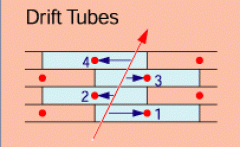
\includegraphics[height=2.5 cm]{../figs/Exp/muonSystem_driftTubes.png}\quad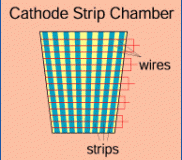
\includegraphics[height=2.5 cm]{../figs/Exp/muonSystem_CSC.png}\quad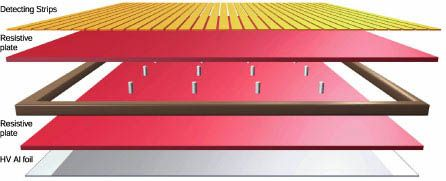
\includegraphics[height=2.5 cm]{../figs/Exp/muonSystem_RPC.png}
    \caption{Components of the CMS muon system. Left to right: drift tubes, cathode strip chambers (CSCs), resistive plate chambers (RPCs).}
    \label{fig:muonSystem}
  \end{center}
\end{figure}


\subsection{Triggering and Data Aquisition}

At peak luminosity, CMS experiences one billion proton-proton collisions per second which come in bunches separated just by~25~ns from one other. New events come before the events from the previous bunch crossing left the detector. To process the information from many different collisions at the same time, data is stored in pipelines. 

It is not technically possible to readout all these events. Moreover, we do not need most of these events for a physics measurement because most of these events do not have a potential to discover a new physics. We have resources to store about one hundred events out of one billion that is why we need a trigger system that quickly decides what the best one hundred events are.

If the triggers were too loose, and we would select one hundred events too quickly, e.g., out of a hundred million events, then CMS would not be able to process the rest~90\% of events in a given set of one billion and we would lose~90\% of potentially interesting events.

If the triggers were too strict, we would select, e.g,~ten events out of one billion, not one hundred and lose CMS potential to store and process data by~90\% which would significantly reduce our chances for a discovery.

Thus, the challenge of the trigger system is to select the best one hundred events out of one billion and do that fast to be able to process every single event. To achive this goal, a two-level trigger system was developed consisting from the Level~1 trigger (L1T) and the high level trigger (HLT) as shown in Fig.~\ref{fig:trigger_2level}.

L1T is a hardware based trigger (Fig.~\ref{fig:trigger_L1}). It uses information from the ECal, HCal and muon system. L1T reduces frequency of coming events from~40~MHz to~100~kHz. Events that did not pass the L1T are lost forever while events that pass the L1T are temporarily stored to get checked by the HLT.

HLT is a software-based trigger. It uses information from all subdetectors and runs quick reconstruction and identification algorithms to determine types of particles and their kinematics. It reduces the number of events to~100~Hz. Events that did not pass HLT are lost forever. Events that pass HLT are arranged into appropriate datasets depending on HLT selection criteria they passed and stored for physics analyses.

\begin{figure}[htb]
  \begin{center}
    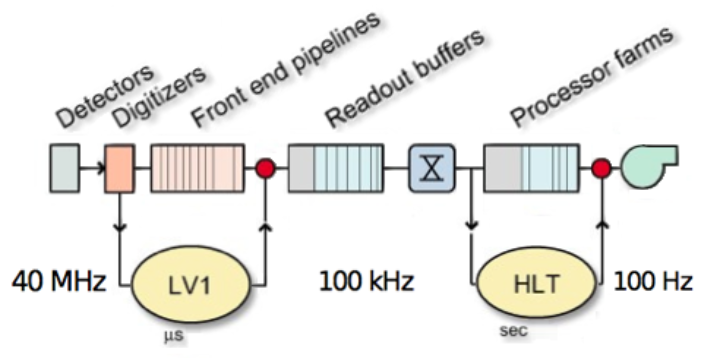
\includegraphics[width=0.8\textwidth]{../figs/Exp/trigger_2level.png}
    \caption{Two-level CMS trigger system.}
    \label{fig:trigger_2level}
  \end{center}
\end{figure}

\begin{figure}[htb]
  \begin{center}
    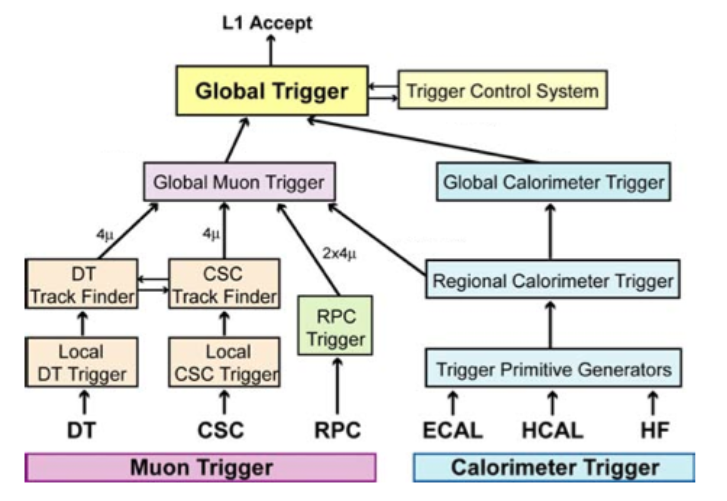
\includegraphics[width=0.8\textwidth]{../figs/Exp/trigger_L1.png}
    \caption{Level 1 CMS trigger system.}
    \label{fig:trigger_L1}
  \end{center}
\end{figure}

\subsection{Particle Flow Algorithm of Event Reconstruction}

A particle flow algorithm is used by CMS to identify and reconstruct stable particles~\cite{ref_ParticleFlowAlg}. It processes the information from all CMS subdetectors and identifies and reconstructs each stable particle in an event individually. The list of particles include muons, electrons, photons, charged and neutral hadrons. Each type of particles leaves its own trace in CMS subdetectors as shown in Fig.~\ref{fig:CMS_slice}. After reconstruction of individual stable particles, jets are built, missing transverse energy $E_T^{miss}$ is determined, certain short-lived particles are reconstructed based on the list of individual stable particles in the event.

One particle can induce several different particle-flow elements in different subdetectors. The linking algorithm links these elements together producing blocks of elements. Usually there are from one to three elements in each block. Links can be connections between the tracking system and silicon strip pre-shower (PS), ECal or HCal, between PS and ECal, between ECal and HCal, and between a tracking system and a muon system. 

In each block, muons are considered first. A link between charged tracks in the tracking and muon systems comprise a global muon which produces one ``particle-flow muon''. The corresponding track in the tracking system is removed from the block and corresponding energy deposits are subtructed from ECal and HCal. Then electrons are reconstructed and identified using tracking system and ECal. The corresponding tracks and ECal clusters are removed from the block. Remaining tracks and clusters are considered more carefully to identify charged hadrons, neutral hadrons, and photons.

When all particles in the event are reconstructed and identified, $E_T^{miss}$ is determined as

\begin{equation}\label{eq:MET}
  E_T^{miss} = - \sum P_T
\end{equation}

where the summation covers all visible particles in the event. $E_T^{miss}$ is used in physics analyses as a measure of $P_T$ of neutrinos and other invisible particles in the event. Fake $E_T^{miss}$ can originate from particles that did not fall into the detector acceptance, particles with very high track curvature that they did not reach the tracking system, momenta mismeasurement, particle misidentification, cosmic rays particles, and machine background.

In the measurement of this dissertation particle flow muons, electrons, photons, and $E_T^{miss}$ are used for all the major steps of the cross section measurement including event selection, background subtruction, various corrections, and determination of phase space restrictions and bin boundaries. Each step is described in greater details in~Ch.~\ref{sec:AN_WgMeas}. 

%Acceptance: particles which are too collinear and go to pipe; particles which get curved too strongly
